\documentclass[aspectratio=169, t]{beamer} % Ratio 16:9
\usepackage[T5]{fontenc}
\usepackage{lmodern}
\usepackage{graphicx} 
\usepackage{array}
\usepackage{longtable} % for long table
\usepackage{chngcntr}
\counterwithin{figure}{section}
\usepackage{tcolorbox}
\renewcommand{\familydefault}{\sfdefault} % Font

\usepackage{caption}
\usepackage{subcaption}
\usepackage{siunitx}

% \definecolor{BlueDefault}{rgb}{0.2,0.2,0.7}
\definecolor{BlueDefault}{RGB}{14,47,95}


% Hide navigation 
\setbeamertemplate{navigation symbols}{}

% Setup background
\newcommand{\normalbackground}{%
    \usebackgroundtemplate{
\includegraphics[width=\paperwidth,height=\paperheight]{Slides/Background/Normal_slide_xPhO.pdf}}%
}

\newcommand{\titlebackground}{%
    \usebackgroundtemplate{
\includegraphics[width=\paperwidth,height=\paperheight]{Slides/Background/Title_slide_xPhO.pdf}}%
}

% Change the title color to white
\setbeamercolor{frametitle}{fg=white} 

% push the title up by \raisebox
\setbeamertemplate{frametitle}{%
    \vspace{0.3em}
    \hspace{-1em} \insertframetitle
    \vspace{2mm}
}

% Number of slide
\setbeamertemplate{footline}{%
    \hfill
    \insertframenumber/\inserttotalframenumber
    \hspace{7.5mm}
    \vspace{3.5mm}
}

%% Make Table of Contents %%
%% Make Table of Contents %%
\AtBeginSubsection[]{
    \begin{frame}
        \frametitle{Mục lục}
        \begin{columns}
            \begin{column}{0.48\textwidth}
                \tableofcontents[sections={1-2}, currentsubsection]
            \end{column}
            \begin{column}{0.48\textwidth}
                \tableofcontents[sections={3-}, currentsubsection]
            \end{column}
        \end{columns}
    \end{frame}
}


%% Section numbering %%
\setbeamertemplate{section in toc}[sections numbered]
\setbeamertemplate{subsection in toc}[subsections numbered]


\renewcommand{\figurename}{Hình}
\renewcommand{\tablename}{Bảng}


%%%%% Bibliography %%%%%
\usepackage[backend=biber,style=ieee]{biblatex}
\addbibresource{myrefs.bib}

\usepackage{url}
\usepackage{hyperref}
\hypersetup{
	colorlinks=true,
	linkcolor=BlueDefault,
	filecolor=BlueDefault,
    citecolor=BlueDefault,
	urlcolor=BlueDefault,
	pdftitle={Overleaf Example},
	pdfpagemode=FullScreen,
}

\begin{document}

\titlebackground

\begin{frame}[noframenumbering]
    \thispagestyle{empty}
    \bfseries
    \begin{flushleft}
        \vfill
        \vspace{5mm}
        \textcolor{BlueDefault}{\huge \bfseries Vector và  \\Nhập môn Đại số tuyến tính} \\
        \vspace{8mm}
        \textcolor{black}{\large \bfseries Người trình bày: Carina }
        \vfill
    \end{flushleft}
\end{frame}

\normalbackground

\section{Tương tác vật lý}
\subsection{Động lượng}
\begin{frame}
\frametitle{Sự thay đổi chuyển động}
\end{frame}
\begin{frame}
\frametitle{Tương tác gần và xa (góc nhìn cổ điển)}
\end{frame}
\begin{frame}
    \frametitle{Khối lượng, Động lượng}
\end{frame}
\subsection{Nguyên lý tương đối}
\begin{frame}
    \frametitle{Của Galilei}
\end{frame}
\section{Ba định luật của Newton}
\subsection{Định luật I}
\begin{frame}
    \frametitle{Định luật quán tính}
    \begin{tcolorbox}[colback=blue!10, colframe=blue!50!black, title=Hệ quy chiếu quán tính]
        Tồn tại một hệ quy chiếu sao cho một vật không chịu tác động của vật khác sẽ chuyển động với vận tốc không đổi (có thể bằng 0).
    \end{tcolorbox}
\end{frame}
\subsection{Định luật II}
\subsection{Định luật III}

\section{Các lực}
\subsection{Các lực cơ bản}

\begin{frame}
    \frametitle{Lực hấp dẫn}
    \begin{tcolorbox}[colback=blue!10, colframe=blue!50!black, title=Định luật vạn vật hấp dẫn]
    Lực hấp dẫn là lực tương tác giữa hai vật có khối lượng, có độ lớn được mô tả bởi công thức:
    \begin{equation}
        F = G \frac{m_1 m_2}{r^2}
    \end{equation}
    trong đó \(G\) là hằng số hấp dẫn, \(m_1\) và \(m_2\) là khối lượng của hai chất điểm, và \(r\) là khoảng cách giữa chúng.
    \end{tcolorbox}
\end{frame}

\begin{frame}
    \frametitle{Lực hấp dẫn}
    \begin{columns}
    \begin{column}{0.5\textwidth}
        \begin{figure}
        \centering
        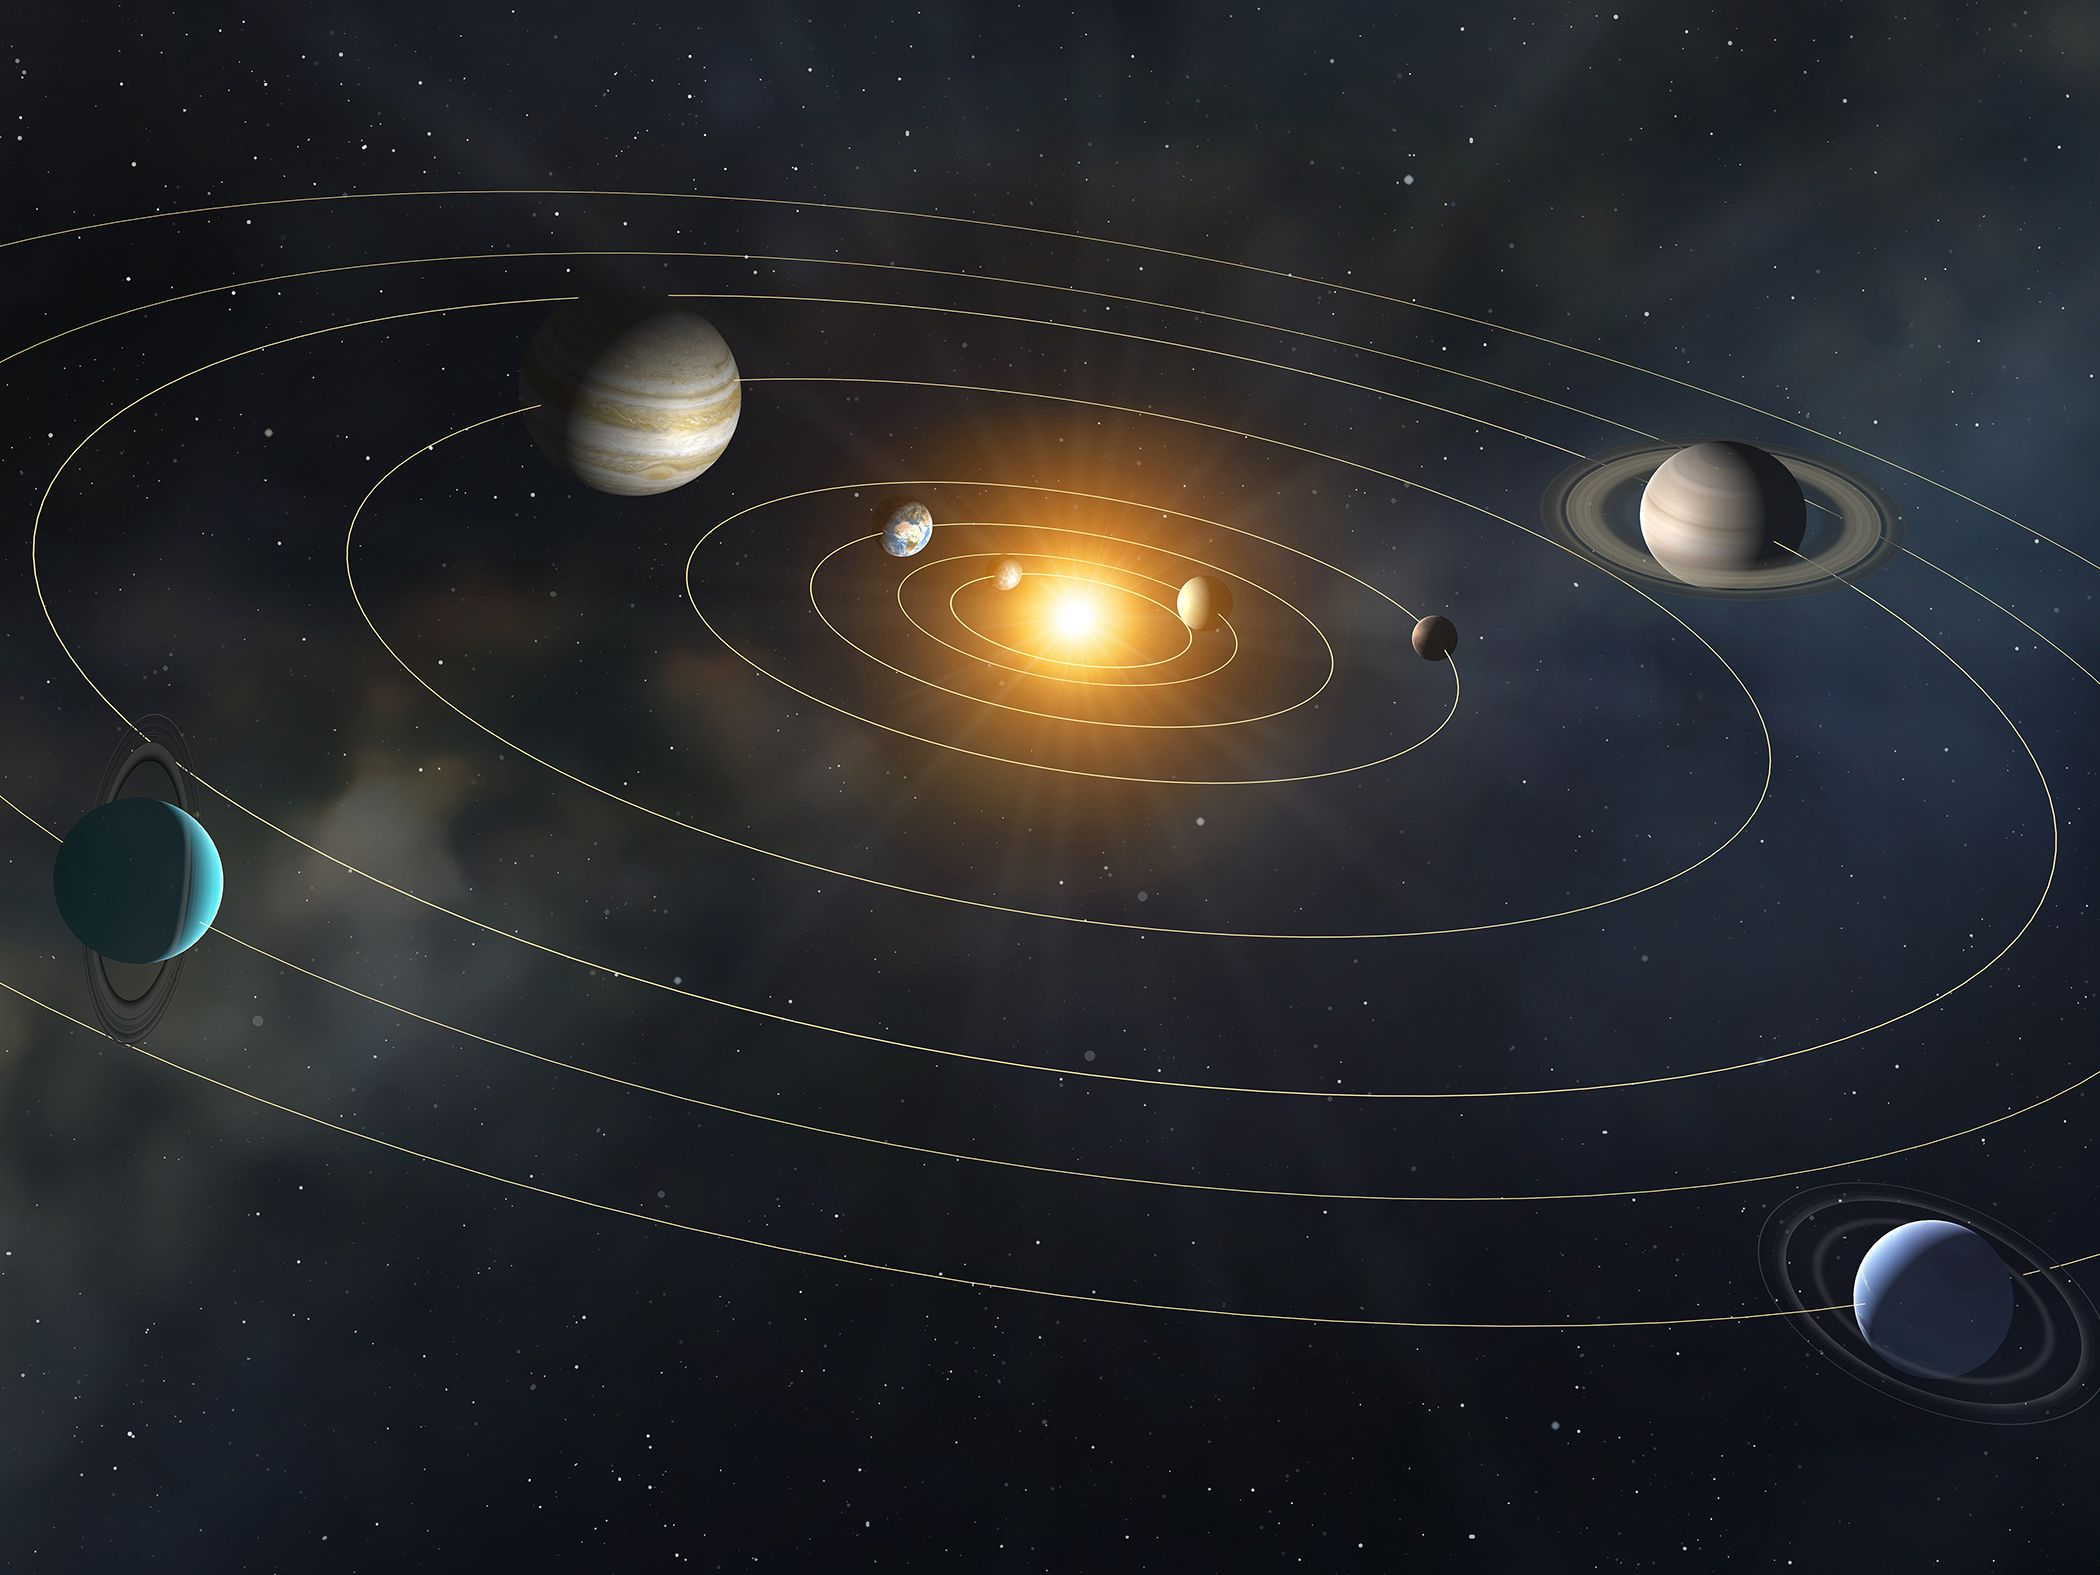
\includegraphics[width=0.8\textwidth,keepaspectratio]{Slides/Figure/solarsystem.jpg}
        \caption{Các hành tinh quay quanh Mặt Trời}
        \end{figure}
    \end{column}
    \begin{column}{0.5\textwidth}
        \begin{figure}
        \centering
        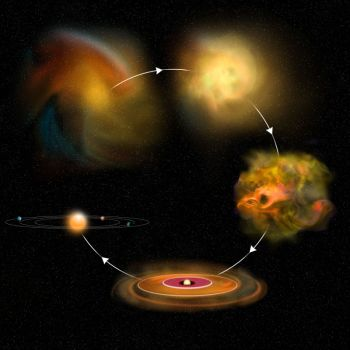
\includegraphics[width=0.6\textwidth,keepaspectratio]{Slides/Figure/planetformation.jpg}
        \caption{Sự hình thành sao và các hành tinh}
        \end{figure}
    \end{column}
    \end{columns}
\end{frame}

\begin{frame}
    \frametitle{Lực hấp dẫn}
    Ở một nơi trên bề mặt trái đất, trọng lực đối với một vật gần như không đổi, có chiều hướng từ trên xuống dưới mặt đất.
    \begin{columns}
    \begin{column}{0.5\textwidth}
        \begin{figure}
        \centering
        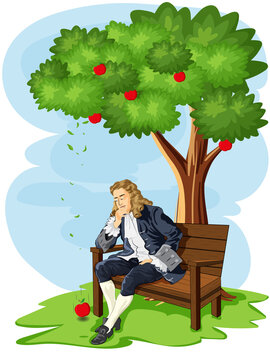
\includegraphics[width=0.4\textwidth,keepaspectratio]{Slides/Figure/applefalling.jpg}
        \caption{Quả táo của Newton rơi do trọng lực}
        \end{figure}
    \end{column}
    \begin{column}{0.5\textwidth}
        Lực này có giá trị bằng:
        \begin{equation}
            F=mg
        \end{equation}
        trong đó \(F\) là lực hấp dẫn, \(m\) là khối lượng của vật, và \(g\) là gia tốc trọng trường (khoảng 9.81 m/s² trên bề mặt Trái Đất).
    \end{column}
    \end{columns}
\end{frame}

\begin{frame}
\frametitle{Lực điện từ}
\begin{tcolorbox}[colback=blue!10, colframe=blue!50!black]
Lực điện từ là lực tương tác giữa các hạt mang điện. Lực này bao gồm lực tĩnh điện, chịu trách nhiệm cho sự hút/đẩy của các điện tích trái dấu/cùng dấu; và lực từ do các điện tích chuyển động tạo ra.
\end{tcolorbox}
Định luật Lorentz \[\mathbf{F}=q(\mathbf{E}+\mathbf{v}\times\mathbf{B}).\]
\begin{figure}
\centering
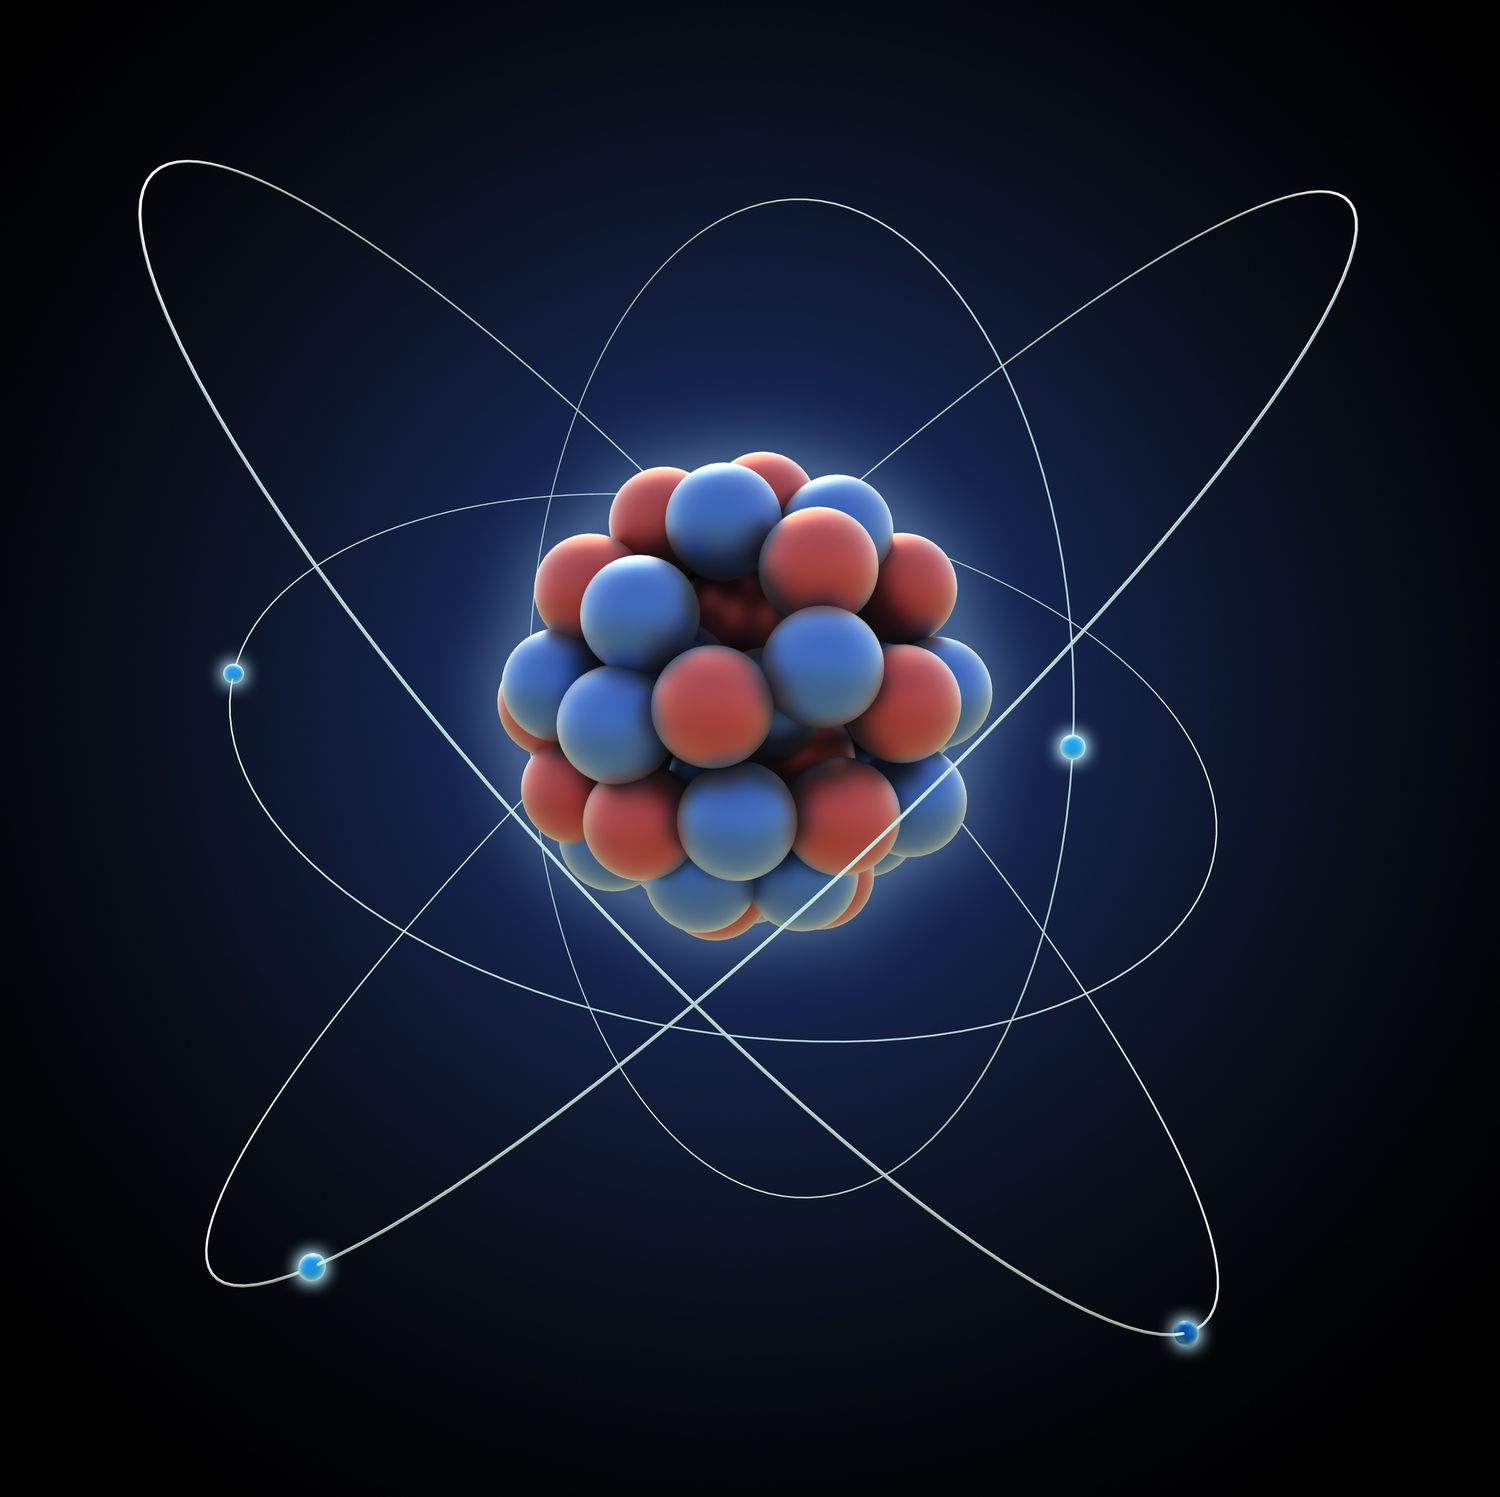
\includegraphics[width=0.15\textwidth]{Slides/Figure/atom.jpg}
\caption{Liên kết giữa các nguyên tử, phân tử}
\end{figure}
\end{frame}

\begin{frame}
\frametitle{Lực điện từ}
\begin{columns}
\begin{column}{0.5\textwidth}
    \begin{figure}
    \centering
    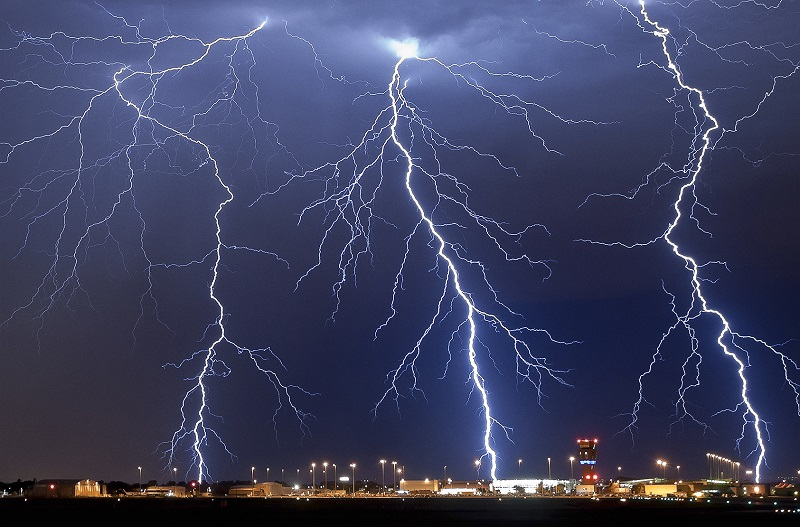
\includegraphics[width=0.775\textwidth]{Slides/Figure/thunder.jpg}
    \caption{Sấm sét}
    \end{figure}
\end{column}
\begin{column}{0.5\textwidth}
    \begin{figure}
    \centering
    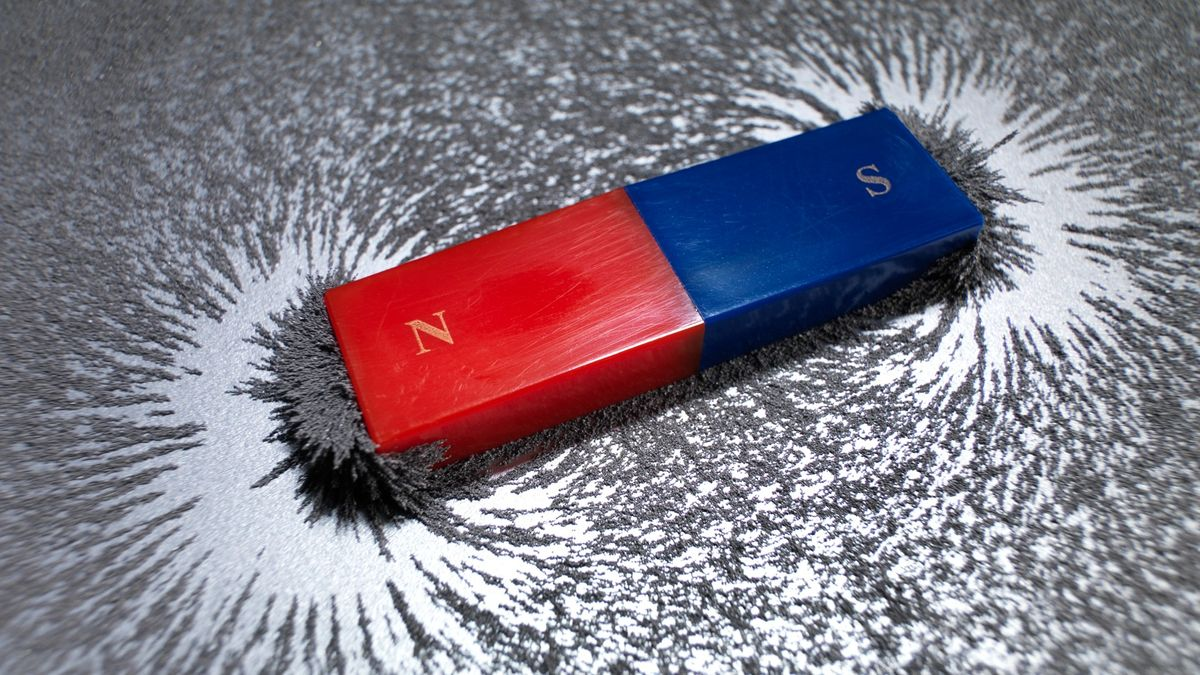
\includegraphics[width=0.9\textwidth]{Slides/Figure/magnet.jpg}
    \caption{Nam châm hút vụn sắt}
    \end{figure}
\end{column}
\end{columns}
\end{frame}

\subsection{Các lực vĩ mô}
\begin{frame}
    \frametitle{Lực đàn hồi}
    \textbf{Lực đàn hồi} xuất hiện khi một vật bị biến dạng và có xu hướng trở về hình dạng ban đầu. Đối với biến dạng không quá lớn, lực này tuân theo định luật Hooke:
    \begin{equation}
        F = -k \Delta x
    \end{equation}
    trong đó \(F\) là lực đàn hồi, \(k\) là hằng số đàn hồi, và \(\Delta x\) là độ biến dạng.
    \begin{figure}
        \centering
        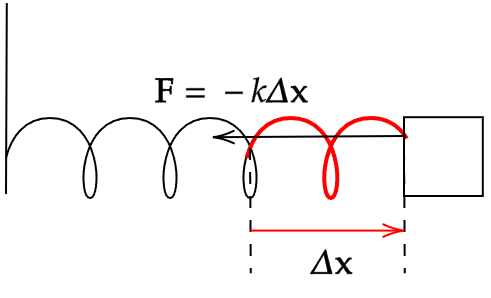
\includegraphics[width=0.3\textwidth]{Slides/Figure/springmass.png}
        \caption{Lực đàn hồi của lò xo}
    \end{figure}
\end{frame}

\begin{frame}
    \frametitle{Lực căng}
    Đối với các vật có hệ số đàn hồi rất lớn, tuy biến dạng nhỏ có thể không quan sát được nhưng vẫn có lực đàn hồi. Lực này gọi là \textbf{lực căng}, thường kí hiệu là \(T\).
    \begin{columns}
    \begin{column}{0.5\textwidth}
        \begin{figure}
        \centering
        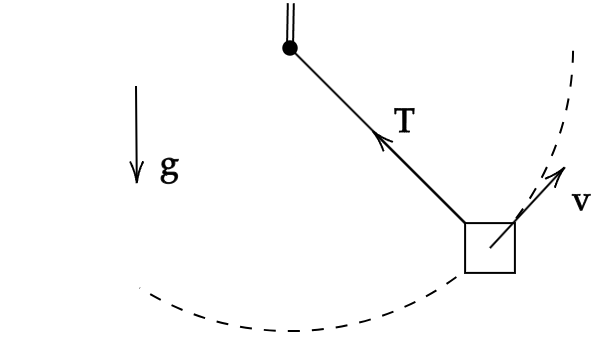
\includegraphics[width=0.6\textwidth]{Slides/Figure/rope.png}
        \end{figure}
        \begin{itemize}
            \item Lực căng dây \(T\) chống lại chuyển động theo phương song song với dây.
    \end{itemize}
    \end{column}
    \begin{column}{0.5\textwidth}
        \begin{figure}
        \centering
        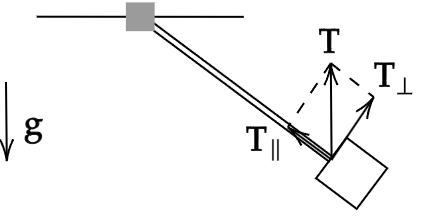
\includegraphics[width=0.5\textwidth]{Slides/Figure/rod.png}
        \end{figure}
        \begin{itemize}
            \item Lực căng thanh \(T_{\parallel}\) chống lại chuyển động theo phương song song với thanh.
            \item Lực căng thanh \(T_{\perp}\) chống lại sự bẻ cong của thanh.
        \end{itemize}
    \end{column}
    \end{columns}
\end{frame}

\begin{frame}
    \frametitle{Phản lực pháp tuyến}
Các mặt phẳng có thể sinh ra lực theo phương pháp tuyến với nó để chống lại sự chuyển động theo phương vuông góc với mặt phẳng này. Lực này được gọi là \textbf{phản lực pháp tuyến}.
\begin{figure}
\centering
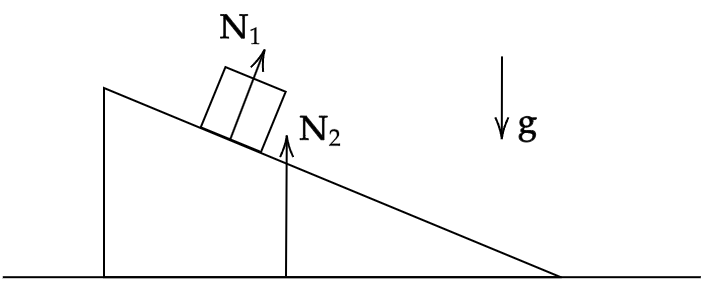
\includegraphics[width=0.5\textwidth]{Slides/Figure/wedge.png}
\caption{Phản lực pháp tuyến của các mặt phẳng}
\end{figure}
\end{frame}

\begin{frame}
    \frametitle{Lực ma sát khô}
    \begin{columns}
    \begin{column}{0.5\textwidth}
    Các khuyết tật trên bề mặt có thể sinh ra phản lực theo phương song song với các bề mặt này khi chúng tiếp xúc với nhau. Lực này được gọi là \textbf{lực ma sát}.
    \begin{figure}
        \centering
        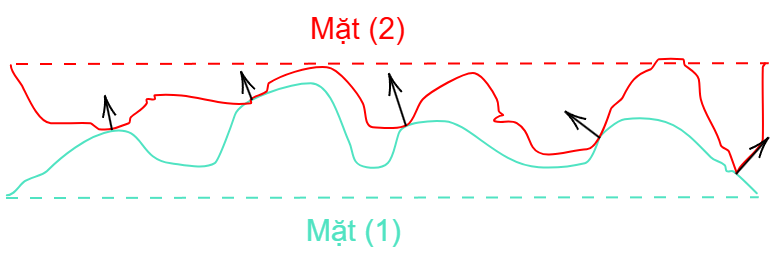
\includegraphics[width=0.9\textwidth]{Slides/Figure/friction.png}
        \caption{Lực ma sát giữa các bề mặt tiếp xúc}
    \end{figure}
    \end{column}
    \begin{column}{0.5\textwidth}
    Lực ma sát khô thường tỉ lệ thuận với phản lực pháp tuyến giữa hai bề mặt:
    \begin{equation}
        F_{ms} = \mu N
    \end{equation}
    trong đó \(F_{ms}\) là lực ma sát, \(\mu\) là hệ số ma sát, và \(N\) là phản lực pháp tuyến.
    \begin{figure}
        \centering
        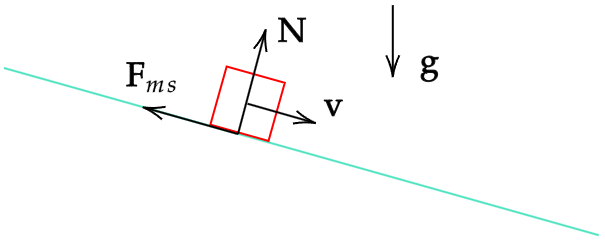
\includegraphics[width=0.7\textwidth]{Slides/Figure/slope.png}
        \caption{Lực ma sát giữa vật và mặt phẳng nghiêng}
    \end{figure}
    \end{column}
    \end{columns}
\end{frame}
\section{Phương pháp}
\subsection{Ba bước giải quyết bài toán}
\begin{frame}{Ba bước giải quyết bài toán}
  \textbf{Bước 1: Quan sát, phân tích thông tin và thiết lập mô hình (nếu cần)}
    \begin{itemize}
        \item Điều cần tìm là gì? Mối liên hệ nào chưa biết?
        \item Có những thông tin nào quan trọng? Những kiến thức nào có thể sử dụng?
        \item Dự đoán hiện tượng.
        \item Tìm cách biến chúng thành phương trình toán học, thiết lập mô hình (nếu cần).
        \item Những đại lượng nào liên quan? Có thể sử dụng phân tích thứ nguyên để dự đoán mối liên hệ không?
  \end{itemize}
\end{frame}

\begin{frame}{Ba bước giải quyết bài toán}
  \textbf{Bước 2: Xử lý bài toán}
    \begin{itemize}
        \item Khảo sát biểu đồ vật tự do.
        \item Dựa vào các thông tin có được (liên kết, định luật, định lý, xấp xỉ…) thiết lập số phương trình tương ứng với số ẩn.
        \item Giải toán.
    \end{itemize}
    \begin{figure}
        \centering
        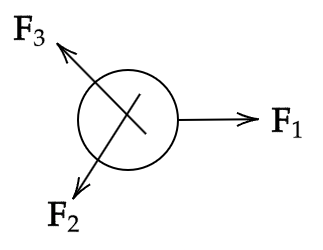
\includegraphics[width=0.25\textwidth]{Slides/Figure/fbd.png}
        \caption{Biểu đồ vật tự do}
    \end{figure}
\end{frame}

\begin{frame}{Ba bước giải quyết bài toán}
  \textbf{Bước 3: Kiểm tra và đánh giá}
    \begin{itemize}
        \item Kiểm tra thứ nguyên của kết quả.
        \item Đối chiếu với các trường hợp đặc biệt, giới hạn.
        \item Quá trình làm có sai sót không? Mô hình lựa chọn có đáng tin cậy không?
        \item Cách tiếp cận cho bài toán là đặc biệt và duy nhất hay có thể đáp ứng cho một loạt các bài toán khác?
        \item Nhận xét ý nghĩa vật lý của lời giải và thử lý giải một cách trực giác.
    \end{itemize}
\end{frame}

\subsection{Ví dụ 1}
\begin{frame}{Ví dụ 1}
Trên một cái nêm khối lượng \(M\) có góc nghiêng \(\alpha\) so với mặt đất đặt một vật có khối lượng \(m\). Hệ số ma sát giữa vật và nêm là \(mu_1\), giữa nêm và mặt đất là \(mu_2\). Tìm gia tốc của vật và nêm.
\begin{figure}
    \centering
    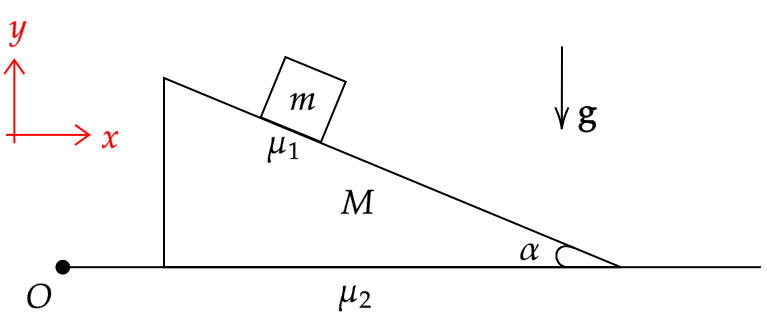
\includegraphics[width=0.5\textwidth]{Slides/Figure/wedgemass.png}
    \caption{Hệ nêm và vật}
\end{figure}
\end{frame}

\begin{frame}{Ví dụ 1}
\begin{columns}
    \begin{column}{0.5\textwidth}
\textbf{Bước 1: Lựa chọn hệ tọa độ phù hợp, phân tích lực.}
\end{column}
    \begin{column}{0.5\textwidth}
\begin{figure}
    \centering
    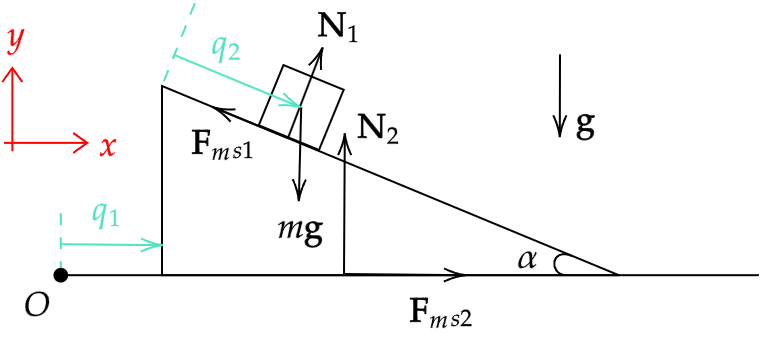
\includegraphics[width=0.8\textwidth]{Slides/Figure/wedgemass1.png}
\end{figure}
\end{column}
\end{columns}
\textbf{Bước 2: Thiết lập hệ 6 phương trình 6 ẩn \(N_1\), \(N_2\), \(F_{ms1}\), \(F_{ms2}\), \(q_1\), \(q_2\).}
\scriptsize
\begin{columns}
\begin{column}{0.4\textwidth}
\begin{align*}
    \begin{cases}
        \mathbf{F_{ms1}}+\mathbf{N_1}+m\mathbf{g}=m\mathbf{a_1} \\
        -F_{ms1}+mg\sin\alpha=m (\ddot q_2+\ddot q_1\cos\alpha) \\
        N_1-mg\cos\alpha=m\ddot q_1\sin\alpha
    \end{cases}
\end{align*}
\end{column}
\begin{column}{0.3\textwidth}
\begin{align*}
    \begin{cases}
        -\mathbf{N_1}-\mathbf{F_{ms1}}+\mathbf{N_2}+\mathbf{F_{ms2}}+M\mathbf{g}=M\mathbf{a_2}\\
        -N_1\cos\alpha-F_{ms1}\sin\alpha+N_2-Mg=0\\
        -N_1\sin\alpha+F_{ms1}\cos\alpha+F_{ms2}=M\ddot q_2
    \end{cases}
\end{align*}
\end{column}
\begin{column}{0.3\textwidth}
\begin{align*}
    \begin{cases}
        F_{ms1}=\mu_1 N_1 \\
        F_{ms2}=\mu_2 N_2
    \end{cases}
\end{align*}
\end{column}
\end{columns}
\normalsize
\end{frame}

\begin{frame}{Ví dụ 1}
    Giải hệ phương trình trên ta được:
    \begin{equation*}
    \ddot q_1 = g\dfrac{M(-\mu_2+\sin\alpha-\mu_1\cos\alpha)\;-\;m\cos\alpha(\mu_1\cos\alpha-\sin\alpha+\mu_2\cos\alpha+\mu_1\mu_2\sin\alpha)}
{m\sin\alpha(\mu_1\cos\alpha-\sin\alpha+\mu_2\cos\alpha+\mu_1\mu_2\sin\alpha)+M(\mu_1\sin\alpha+\cos\alpha)}
    \end{equation*}
    \begin{equation*}
        \ddot q_2 = g\dfrac{M(\mu_2\cos\alpha+\mu_1\mu_2\sin\alpha)\;+\;m(\mu_1\cos\alpha-\sin\alpha+\mu_2\cos\alpha+\mu_1\mu_2\sin\alpha)}
{m\sin\alpha(\mu_1\cos\alpha-\sin\alpha+\mu_2\cos\alpha+\mu_1\mu_2\sin\alpha)+M(\mu_1\sin\alpha+\cos\alpha)}
    \end{equation*}
\textbf{Bước 3: Kiểm tra và đánh giá}
\begin{itemize}
    \item Kiểm tra thứ nguyên: \([ML^2T^{-2}]\) của gia tốc.
    \item Việc gọi ra các lực liên kết như \(N_1\), \(N_2\) có thể áp dụng được cho một loạt bài toán khác.
\end{itemize}
\end{frame}

\subsection{Ví dụ 2}
\begin{frame}{Ví dụ 2}
    Một quả cầu có khối lượng \(m\), thể tích \(V\) được nhúng trong một chất lỏng có khối lượng riêng \(\rho\). Khi di chuyển ở trong chất lỏng, vật chiu một lực cản nhớt \(\mathbf F_c=-k\mathbf v\). Biết rằng ban đầu vật xuất phát tại gốc tọa độ với vận tốc \(mathbf v_0\) theo phương x. Tìm tọa độ của vật theo thời gian.
\begin{figure}
    \centering
    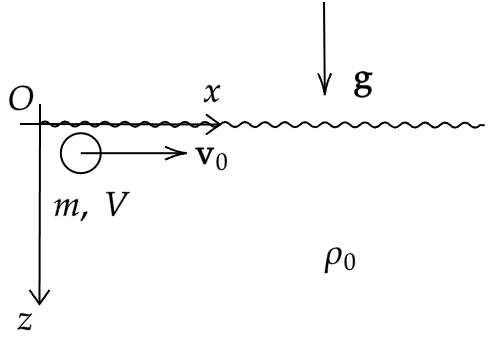
\includegraphics[width=0.4\textwidth]{Slides/Figure/masatnhot.png}
\end{figure}
\end{frame}

\begin{frame}{Ví dụ 2}
\begin{columns}
    \begin{column}{0.5\textwidth}
\textbf{Bước 1: Phân tích lực.}
\end{column}
    \begin{column}{0.5\textwidth}  
\begin{figure}
    \centering
    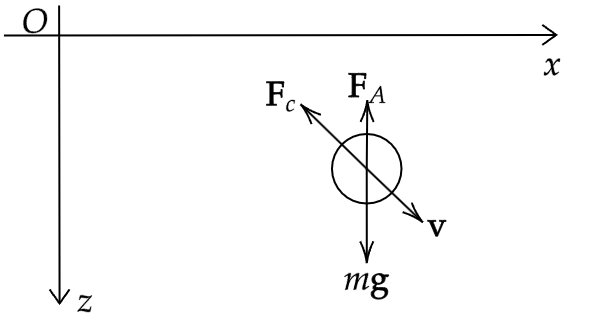
\includegraphics[width=0.7\textwidth]{Slides/Figure/masatnhot1.png}
\end{figure}
\end{column}
\end{columns}
\textbf{Bước 2: Thiết lập hệ phương trình 2 ẩn \(x\), \(y\) từ \(m\mathbf a=\mathbf F_c+\mathbf F_A+m\mathbf g\).}
\scriptsize
\begin{columns}
\begin{column}{0.5\textwidth}
\begin{align*}
    \text{Phương x:}\quad
    \begin{cases}
    m\ddot{x} = -k\dot{x}. \\
    m\int_{v_0}^{\dot{x}} \dfrac{d\dot x}{\dot x} = -k\int_0^t dt. \\
    \dot x=v_0 \exp(\dfrac{-kt}{m}).
    \end{cases}
\end{align*}
\end{column}
\begin{column}{0.5\textwidth}
\begin{align*}
    \text{Phương z:}\quad
    \begin{cases}    
    m\ddot{z} = -\rho g V + mg - k\dot{z}. \\
    m\int_{0}^{\dot z} \dfrac{d(k\dot z+\rho g V-mg)}{k\dot z+\rho g V-mg} =-k\int_0^t dt.\\
    \dot{z} = \left(\dfrac{mg - \rho g V}{k}\right)\left[1 - \exp\left(-\frac{k t}{m}\right)\right]
    \end{cases}
\end{align*}
\end{column}
\end{columns}
\normalsize
\end{frame}

\begin{frame}{Ví dụ 2}
Tích phân theo thời gian 2 phương tình trên:
\begin{equation*}
    x(t) = \dfrac{m}{k}v_0\left(1 - \exp\left(-\dfrac{kt}{m}\right)\right)
\end{equation*}
\begin{equation*}
    z(t) = \dfrac{mg - \rho g V}{k}t - \dfrac{m}{k}\left(\dfrac{mg - \rho g V}{k}\right)\left[1 - \exp\left(-\dfrac{kt}{m}\right)\right]
\end{equation*}
\textbf{Bước 3: Kiểm tra và đánh giá}
\begin{itemize}
    \item Kiểm tra thứ nguyên: \([L]\) của tọa độ.
    \item Khi \(m\to\infty\) hoặc \(k\to 0\), từ khai triển Taylor: \(x(t)\approx v_0 t\) và \(z(t)\approx \frac12 g t^2\).
    \item Khi trọng lực bằng lực đẩy Archimedes: \(z(t)=0\).
\end{itemize}
\end{frame}
\begin{frame}[allowframebreaks]{Tài liệu tham khảo}
    \begin{refsection}
        \nocite{morin2008introduction,calculusjame, 3b1b,griffiths2023introduction}
         \printbibliography
    \end{refsection}
\end{frame}

\end{document}